% !TEX root = ../../AdvStaDaAn.tex
\section{Model Fitting}
\subsection{Akaike's Information Criterion (AIC)}
Weights \glqq goodness-of-fit\grqq{} against the complexity of the model.
\begin{align*}
\text{AIC}
=
-2 (\text{maximized log-likelihood})
+ 2\;\text{\#estimated parameters}
\end{align*}
and for linear regression model
\begin{align*}
\text{AIC}
=
n \log\left(\frac{1}{n}\sum_{i=1}^n\right) + 2 p^\diamond + \text{constant}
\end{align*}
where $p^\diamond$ is the number of parameters,
i.e.,
including $\widehat{\sigma}$.

\subsection{Test Statistic}
To assess the contribution of a group of $q$ explanatory variables to the
model,
we study the test statistic
\begin{align*}
F
=
\frac{(SS_E^* - SS_E)/q}{SS_E/(n-p)}
=
\frac{(SS_E^* - SS_E)/q}{\widehat\sigma^2}
\end{align*}
where
\begin{itemize}
\item $SS_E^*$ is the sum of the squared residuals
of the \glqq reduced\grqq{} model (=null hypothesis $H_0$)
\item $SS_E$ is the sum of the squared residuals
of the \glqq full\grqq{} model (=alternate hypothesis)
\end{itemize}

\subsection{Datasets}
Ideally, the data for construction of a prediction function (i.e., the learning
set) and the future cases to be predicted are, in some sense, a \textit{sample}
from a \textit{well-defined} population.
\begin{itemize}
\item Often, however, one cannot guarantee these conditions
\begin{itemize}
\item For example, if the experiment were done in one day, or by one
technician, or in one laboratory.
\item Or, the learning sample is by design representative of only a small
segment of a larger population
\end{itemize}
\end{itemize}

\subsection{Fitting Smooth Functions}

\subsubsection{Locally Weighted Regression (LOWESS / LOESS)}
LOESS is based on local parametric regressions
\begin{enumerate}
\item Choose a window with fixed with $2b_w$ around a point $x$
\item Within this window a straight line is fitted to the data
\item Predict value in the window center = value of the smoother
\item Repeat (1) to (3) for a set of $x$-values
\item To visualize the smoother,
the points are connected by straight line segments
\end{enumerate}
Regression fitting downweights the data with respect to their distance from the
window center.
In the estimator one can controll
\begin{itemize}
\item type of regression (constant, linear or quadratic)
\item fitting algorithm (least squares or robust)
\item neighbourhood size $b_w$
\end{itemize}

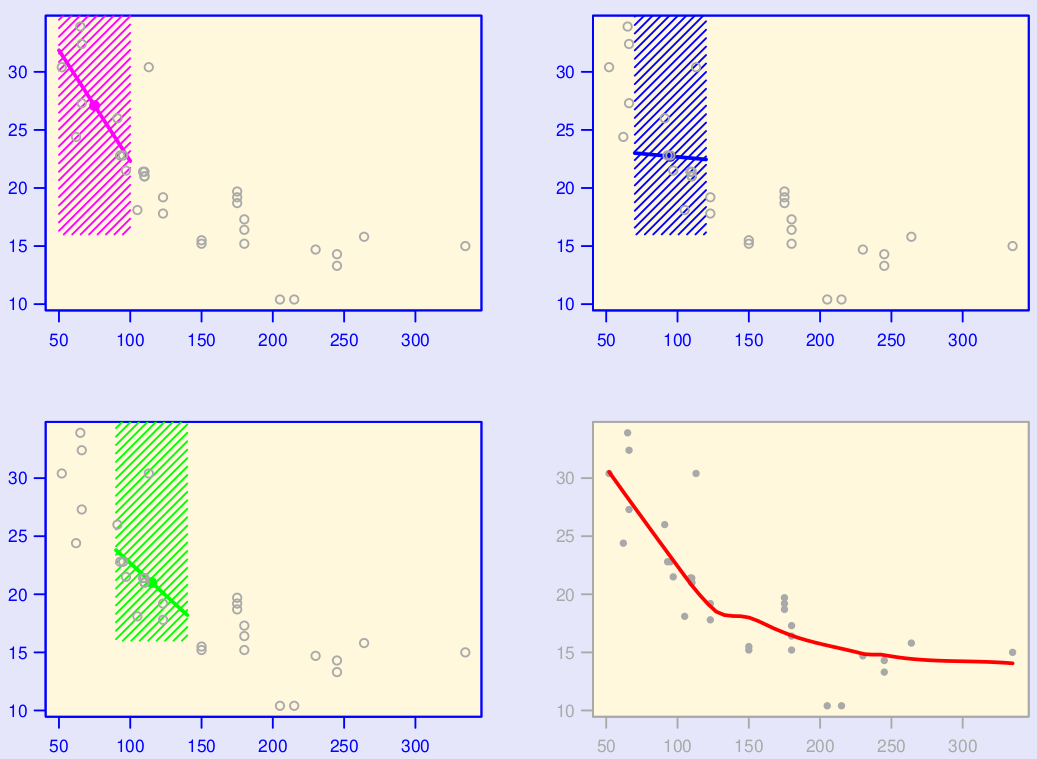
\includegraphics[width=0.7\textwidth]{sections/ModelFitting/images/loess.png}

\subsubsection{Cubic Spline Smoothing}
Linear combination of some basis function $h_m$, $m=1,\ldots,M$
\begin{align*}
f(x) = \sum_{m=1}^M \gamma_m h_m(x)
\end{align*}
\begin{itemize}
\item The basis functions $h_m$ are known
\item The $\gamma_m$ are some unknown parameters that are to be determined
from the data (e.g. by the OLS method)
\item The number $M$ controls the smoothness and,
the complexity of $f(x)$,
i.e. the adaptation to the \glqq true\grqq{} function underlying the data.
\end{itemize}
Preventing overfitting by minimizing
\begin{align*}
\sum_{i=1}^n (y_i - f(x_i))^2 + \lambda \cdot \text{\glqq roughness\grqq{}}
\end{align*}

\subsection{Additive Regression Model}
The possibility of estimating a functional relationship nonparametrically
allows a more general formulation of the regreesion model,
known as \textbf{(generalised) additive model}.
\begin{align*}
Y_i
=
\beta_0 + \sum_{j=1}^m f_m(x_i^{(j)}) + E_i
,\quad
\text{with $E$ independent}
\sim \mathcal{N}(0, \sigma^2)
\end{align*}
\begin{itemize}
\item Goal is to fit a flexible component $f_k$ for each predictor $x_i^{(k)}$
\item Can be achieved by, e.g. cubic splines with automatic estimation of the
correct complexity
\item These flexible functions $f_k$ are transformations of $x^{(k)}$
\end{itemize}

\subsection{Model Building}
\begin{enumerate}
\item Clarify the task (purpose? goal? prediction vs exploration);
are there already model approaches?
\item Data Screening and Processing
\item Set up model using Tukey’s first-aid transformations or GAMs
\item Model fitting; preferably with robust methods
\item Residual and sensitivity analysis;
does this dataset help solving the task?
\newline
Eventually back to (3), (2) or (1)
\item Variable selection; treat collinearities if necessary
\newline
Eventually back to (3)
\item Checking model adequacy
\begin{itemize}
\item Residual and sensitivity analysis with selected model(s)
\item Check plausibility; match model(s) with subject matter expertise
\item Out-of-sample validation, especially if the model is to be used for
prediction
\end{itemize}
Eventually back to (1), (2), (3), $\ldots$
\item Reporting:
It is key to be honest and openly report all data manipulations and
decisions that were made.
\end{enumerate}